\InputIfFileExists{../data/global.src}\relax\relax

\iffull
\definecolor{@joda}{RGB}{204, 186, 157}
\definecolor{@joda@}{RGB}{78, 68, 66}
\setbox\pinguA=\hbox{\tikz\pingu[body=pingu@green!52!pingu@black,body front=pingu@green!52!pingu@black!5!pingu@white,cloak=@joda,cloak cap=@joda,lightsaber right=pingu@green,lightsaber right length=1.4cm,shirt=@joda@,shirt no buttons,small,eyes wink,cane left=pingu@bronze!80!pingu@black,cane left length=11mm,cane left raise=1mm,right item angle=-30];}
\titlesuffix{\tikzpicture[overlay,remember picture]
    \node[above left,yshift=\btdmfootheight-1mm] at(current page.south east) {\copy\pinguA};
\endtikzpicture}
\def\packtitlenode#1#2{\node[font=\usebeamerfont{title},inner xsep=0pt,opacity=#1,outer ysep=2pt] (#2) {getauscht};}
\title[Erstes Tutorium -- Übungsblatt 2]{Diese Worte \texorpdfstring{\,\setbox0=\hbox{getau\kern5pt\relax scht}\phantom{\copy0}\llap{\tikz[baseline=(k.base)]{%
\packtitlenode0k
\def\kA{310}\def\kB{130}\def\kS{-.5\wd0-5pt}
\scope[xshift=-\kS]\packtitlenode0x
\clip (x.south west)--(x.\kA)--(x.\kB)-| cycle;
\packtitlenode1x
\endscope
\scope[xshift=\kS]
\packtitlenode0y
\clip (y.south east)--(y.\kA)--(y.\kB)-| cycle;
\packtitlenode1y
\endscope
% cutline
\fill[btdm@border@down,rounded corners=1.5pt] ([yshift=4pt,xshift=1.5pt]y.\kA)--([yshift=-4pt]y.\kB)--++(-3pt,0)--([xshift=-1.5pt,yshift=4pt]y.\kA) -- cycle;
\fill[btdm@border@down,rounded corners=1.5pt] ([yshift=4pt,xshift=-1.5pt]x.\kA)--([yshift=-4pt,xshift=-1.5pt]x.\kB)--++(3pt,0)--([xshift=1.5pt,yshift=4pt]x.\kA) -- cycle;
}\kern-.5\wd0}\;~}{getauscht} ich habe}
\subtitle{Tutorium Zwei}
\date{KW 19}
\addbibresource{references.bib}
\fi
\SetTutoriumNumber{2}

\iffull\begin{document}
\titleframe

\TopicOverview{2}
\fi

\iffull{\SummaryFrame
\def\sub#1#2{\node[font=\tiny\sffamily,align=center,gray,below=-3mm] at(#1.south) {\strut#2\strut};}
\begin{frame}[fragile,c]{Kurzwiederholung}
    \begin{itemize}[<+(1)->]
        \itemsep14pt
        \item Algorithmenkonstruktion\smallskip\par \centerline{%
            \begin{tikzpicture}
                \onslide<+(1)->\node (0) at(0,0) {\strut Spezifikation};
                \sub0{Begriffe mit\\Problemrelevanz}
                \foreach[count=\i,remember =\i as \li (initially 0)] \a/\t in {Abstraktion/{Gegeben \& Gesucht},{\sbseries Entwurf}/{Algorithmus},Verifikation/{Termination \&\\partielle Korrektheit},Aufwandsanalyse/{Laufzeitverhalten}} {
                    \onslide<+(1)->\node[right=.5mm] (k\i) at(\li.east) {\strut\faAngleRight};
                    \node[right=.5mm] (\i) at (k\i.east) {\strut\a};
                    \sub\i{\t}
                }
            \end{tikzpicture}}\vspace*{-\medskipamount}
        \item Kerneigenschaften eines Algorithmus: \begin{itemize}
            \item Von einem Prozessor \info{Mensch,~\ldots} in endlich vielen Schritten Ausführ- und Reproduzierbar
            \item Eine endliche Beschreibung in Elementaroperationen.
        \end{itemize}
        \item Abstrakte Variablenoperationen:
\begin{plainjava}
!*\onslide<12->*!long x; !*\tikzmarknode{@1}{\phantom{Ig}}*!
!*\onslide<12->*!x = 21; !*\tikzmarknode{@2}{\phantom{Ig}}*!
!*\onslide<12->*!x = 42; !*\tikzmarknode{@3}{\phantom{Ig}}*!
\end{plainjava}
    \end{itemize}
\begin{tikzpicture}[overlay,remember picture,T/.style={sol@colors@lst@comments,font=\itshape\sffamily\footnotesize}]
\onslide<13->{\node[right,T] at(@1.east) {\textbf{Deklaration} --- Reservieren von Namen mit Typ long};}
\onslide<14->{\node[right,T] at(@2.east) {\textbf{Initialisierung} --- Erste Wertzuweisung, macht die Variable verwendbar};}
\onslide<15->{\node[right,T] at(@3.east) {\textbf{Wertzuweisung} --- Überschreiben/Ändern des vorherigen Wertes};}
\end{tikzpicture}
\end{frame}
}\fi

\SetNextSectionText{\say{Machs Farbig}\\--- Isabell Bannweg}
\def\HStrut{\vphantom{\{\}}}
\section{Exkurs: Parameter}
\begin{frame}[fragile]{M-Array me und andere Zukunftsträume}
    \begin{itemize}[<+(1)->]
        \itemsep8pt
        \item Arrays werden später genauer behandelt.
        \item Arrays sind Listen fester Größe die Elemente des gleichen Datentyps beinhalten.
        \item Wir notieren sie mit \T{[]}:
\begin{plainjava}[lineskip=1.25pt]
!*\onslide<5->*!int!*\tikzmarknode{@}{\solGet{basicstyle}{\HStrut[]}}*! arr = {42, !*\tikzmarknode{@2}{\solGet{basicstyle}{\solGet{numbers}{\HStrut-7}}}*!,  !*\tikzmarknode{@4}{\solGet{basicstyle}{\solGet{numbers}{\HStrut13}}}*!};

!*\onslide<7->*!System.out.println(!*\tikzmarknode{@3}{\solGet{basicstyle}{arr[\solGet{numbers}{\HStrut1}]}}*!);!*\onslide<9->*! // :yields: -7

!*\onslide<10->*!System.out.println(!*\tikzmarknode{@5}{\solGet{basicstyle}{arr[arr.length - \solGet{numbers}{\HStrut1}]}}*!); !*\onslide<12->*!// :yields: 13
\end{plainjava}
    \end{itemize}
\begin{tikzpicture}[overlay,remember picture,codeouthl]
    \def\hlhs{0mm}
    \onslide<6->{
        \hlcode[-.35pt]{@}{array}
        \draw[Kite-] (@.south) to[out=290,in=180] ++(1,-.35) node[right] {\small\itshape Ein Array an Integern.};
    }
    \onslide<8->{
        \def\hlopa{.6}
        \def\hlcolor{pingu@yellow}\hlcode[-.35pt]{@2}{-7}
        \hlcode[-.35pt]{@3}{1}
        \node at(@2) {\solGet{basicstyle}{\solGet{numbers}{\HStrut-7}}};
        \node at(@3) {\solGet{basicstyle}{\HStrut arr[\solGet{numbers}{1}]}};
    }
    \onslide<9->{\draw[Kite-] (@3.330) to[out=240,in=0] ++(-1,-.25) node[left] {Beginnt bei \(0\)};}
    \onslide<11->{
        \def\hlopa{.6}
        \def\hlcolor{pingu@green}\hlcode[-.35pt]{@4}{13}
        \hlcode[-.35pt]{@5}{1}
        \node at(@4) {\solGet{basicstyle}{\solGet{numbers}{\HStrut13}}};
        \node at(@5) {\solGet{basicstyle}{\HStrut arr[arr.length - \solGet{numbers}{1}]}};
    }
    \onslide<12->{\draw[Kite-] (@5.280) to[out=240,in=0] ++(-1,-.3) node[left] {Liefert die Array-Größe (3)};}
\end{tikzpicture}
\end{frame}

\begin{frame}{Die Sache mit dem \T{String[] args}}
 % TODO: arrays,
 % TODO: Kommandozeilenparameter
 % TODO: AAAAAAAAAAAAAH
\end{frame}

\SetNextSectionText{Es gibt keine if-Schleifen, sondern nur if-Abfragen!\\--- \href{http://if-schleife.de/}{if-schleife.de}}
\section{Präsenzaufgabe}
\begin{frame}[fragile,c]{Präsenzaufgabe}
\begin{aufgabe}{Wenn\ldots\ Ja wenn nur die Schleife nicht wär\ldots}
    \onslide<2->{Legen Sie eine Java Datei namens \T{ErsteSchleife.java} an \info{oder bearbeiten Sie die Aufgabe auf einem Blatt Papier}.} \onslide<3->{Lesen Sie in der main Methode eine \bjava{int} Variable namens \(n\) über die Kommandozeilenparameter ein und implementieren Sie eine for Schleife, die jede dritte Zahl von \(1\) bis einschließlich \(n\) ausgibt.}
    \onslide<4->Beispiel:
\begin{plainjava}
n = 13 !*\onslide<+(1)->*!// :yields: 1 4 7 10 13
\end{plainjava}
\onslide<1->
\end{aufgabe}
\end{frame}

\begin{frame}{}

\end{frame}

\section{Abschließendes}
{\SummaryFrame
\begin{frame}[t]{Zusammenfassend}
\pause \printBibCommand
\vfill\vfill % double fill for more fraction
\begin{itemize}[<+(1)->]
    \itemsep14pt
    \item Wir haben die Geburt von Variablen sowie ihre Wachstumsphase kennengelernt: \begin{itemize}
        \item Die \textit{Deklaration} (\bjava{int x}) reserviert einen Namen samt Charakteristika (Typ,~\ldots)
        \item Die \textit{Initialisierung} (\bjava{int x; x = 5}) beschreibt die erste Wertzuweisung
        \item Eine \textit{(Wert-)Zuweisung} (\bjava{x = 3}) ist jede weitere Änderung des gespeicherten Wertes
    \end{itemize}
    \item In die Wahl des \say{richtigen\texttrademark} Datentyps fließen viele Informationen mit ein.
\end{itemize}
\end{frame}
}

\outro{\vskip6mm\centering\begin{tikzpicture}[scale=2.5]
    % \only<2->{\pingu[monocle left,right eye wink,left eye vertical,laptop right,cane left,tie,body type=legacy,headphones=pingu@green!80!pingu@black]}
    % TODO
\end{tikzpicture}}


\iffull\end{document}\fi
